\section{Discussion} \label{sec: discussion}
\rev{The RDMA framework addresses critical bottlenecks in clinical information extraction by leveraging the adaptability of agentic workflows. This section explores the strengths of our approach, the persistent challenges of medical reasoning, and the need for more robust benchmarking in rare disease research.}

\begin{wraptable}{r}{0.45\textwidth}
    \centering
    \small 
    \vspace{-15pt} % Adjust this value as needed
    \begin{tabular}{lccc}
        \toprule
        \textbf{\rev{Baseline}} & \textbf{\rev{F1}} & \textbf{\rev{P}} & \textbf{\rev{R}} \\
        \midrule
        \rev{RDMA} & \rev{\textbf{0.65}} & \rev{0.63} & \rev{0.68} \\
        \rev{No Lab Tool} & \rev{0.64} & \rev{0.63} & \rev{0.64} \\
        \rev{No Impl. Check} & \rev{0.65} & \rev{\textbf{0.64}} & \rev{0.65} \\
        \rev{No Verif.} & \rev{0.53} & \rev{0.42} & \rev{\textbf{0.71}} \\
        \bottomrule
    \end{tabular}
    \caption{\rev{\textbf{RDMA Ablation Study.} Impact of individual components on phenotype mining performance of a quantized Mistral 24B model on the CSC \cite{garcia2024_HPORAG}.}}
    \label{tab:rdma_ablation}
    \vspace{-20pt} 
\end{wraptable}

\rev{\textbf{The flexibility of agentic frameworks.} A key advantage of agentic frameworks over fixed pipelines is their task-specific adaptability. As shown in Fig. \ref{fig:RDMAvRAG}, phenotype and disease extraction agents utilize distinct tools while maintaining a shared workflow of extract, verify, match, and refine. RDMA allows for modular customization—such as including abbreviation detection or lab event databases for phenotype extraction while omitting lab events for rare disease extraction, where they provide no value. Our ablation study (Table \ref{tab:rdma_ablation}) underscores the importance of this modularity. While the lab test tool and implication reasoning provide marginal gains in recall, the \textbf{verification step} is the most critical component, providing a substantial boost to precision by filtering out hallucinations and misalignment.}

\rev{\textbf{Challenges in phenotype mining and medical reasoning.} Despite the strengths of agentic systems, significant challenges remain in capturing \textbf{implied phenotypes}. Analysis of our benchmark (Fig.~\ref{fig:DatasetBreakdown}) reveals that over 25\% of phenotypes are not explicitly mentioned in the text. These require LLMs to infer conditions from lab results or symptom clusters. Current LLMs remain insufficient for basic reasoning tasks like implying phenotypes related to lab events, as shown by the tiny improvements in Fig.~\ref{fig:DatasetBreakdown}. RDMA still struggles with: (1) \textit{Long-context reasoning}: failing to link distal mentions (e.g., a colonoscopy performed earlier in a note to a ``colonic tubular adenoma''); (2) \textit{Terminology nuance}: identifying ``decreased visual acuity'' as a match for the HPO code ``reduced visual acuity''; and (3) \textit{Negation detection}: occasionally ignoring negative qualifiers (e.g., ``negative for...''), even when prompted to consider negations.}

\begin{figure}[h!]
    \centering
    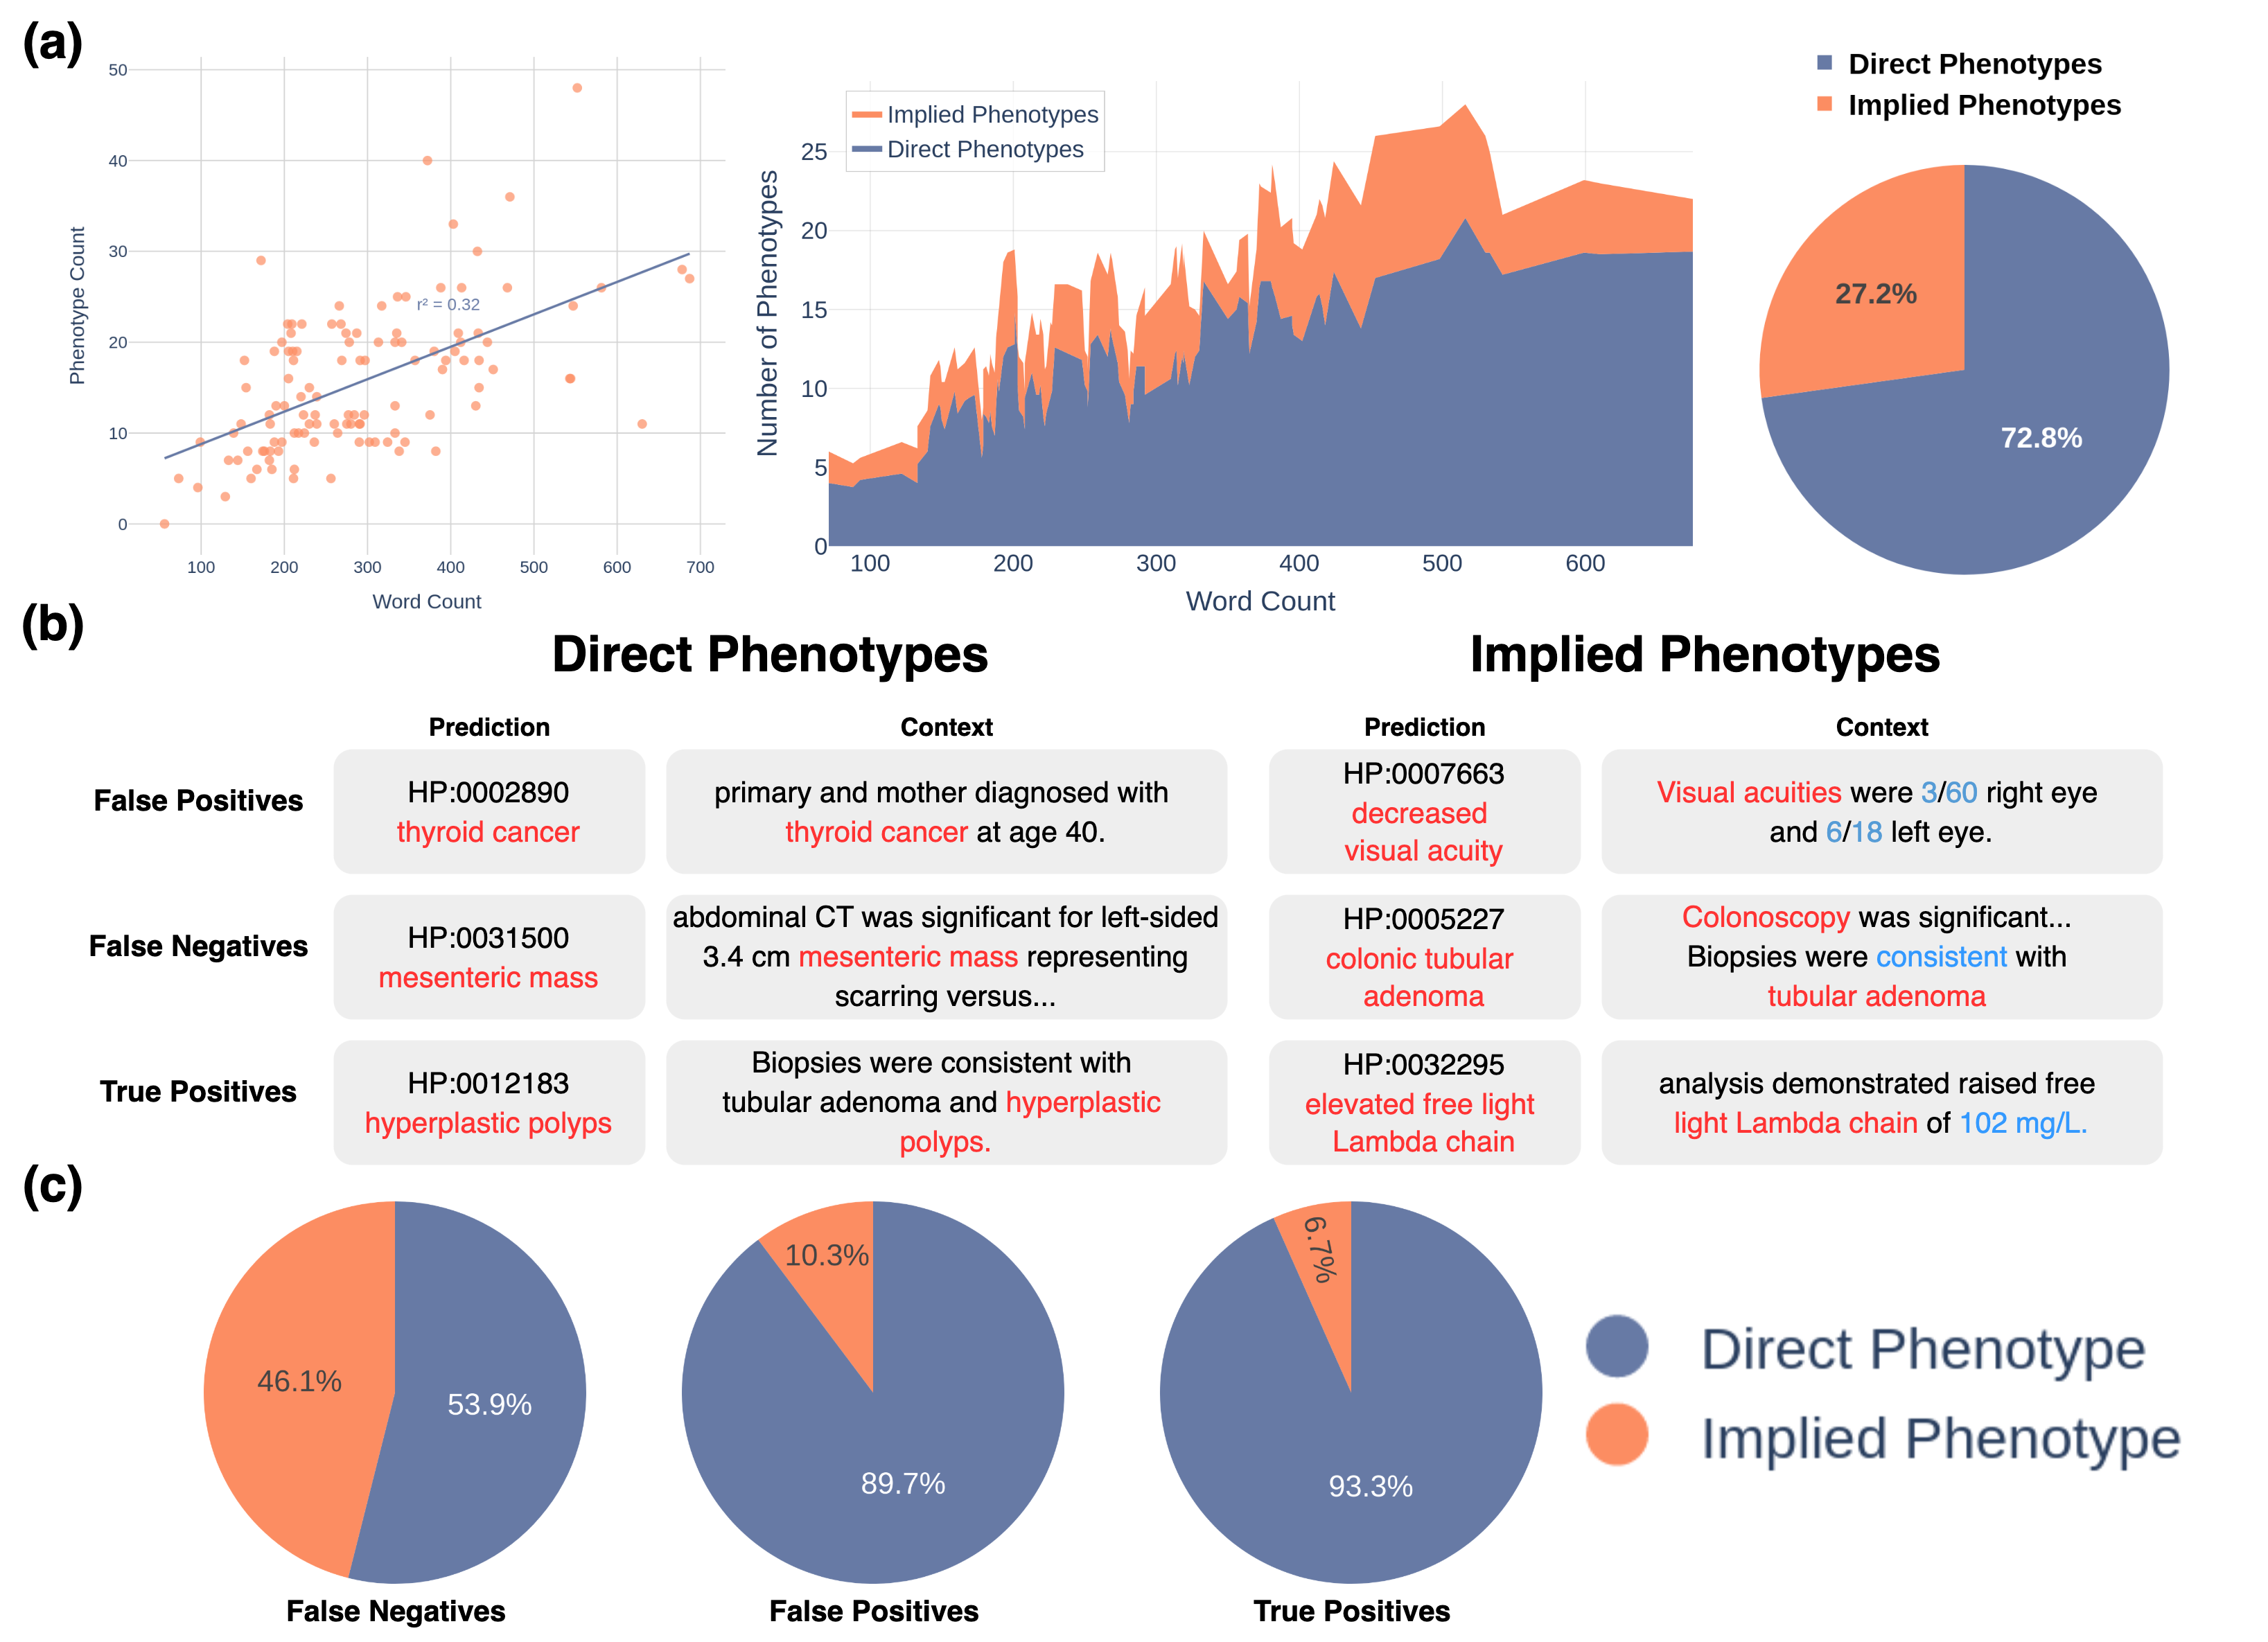
\includegraphics[width=1.0\textwidth]{figs/PhenotypeQualitativeEvaluationsAndStatistics.drawio.png}
    \caption{}
    \label{fig:DatasetBreakdown}
\end{figure}

\rev{\textbf{Robustness to clinical note complexity.} A primary hurdle in rare disease mining is the discrepancy between scientific passages and real-world EHRs. Clinical notes in datasets like MIMIC-IV are often thousands of words long and laden with noise such as abbreviations and misspellings. As shown in Fig. \ref{fig:RDMA_Note_Lengths}, RDMA demonstrates remarkable robustness to document length. Unlike one-shot RAG approaches that typically perform a single extraction and degrade as context grows, RDMA’s recall slightly increases with longer texts. By retrieving against individual sentences and employing agentic verification, we maintain a stable F1 score across varying lengths. Nonetheless, a great area of interest is improving the ability of these systems at longer and noisier contexts, especially given that the performance discrepancy of approaches on the scientifc RareDis corpus and our cleaned MIMIC3 clinical note corpus has a gap of over 20\% F1 as shown in Table \ref{tab:main_results_combined_v3}.  }

\begin{figure}[h!]
    \centering
    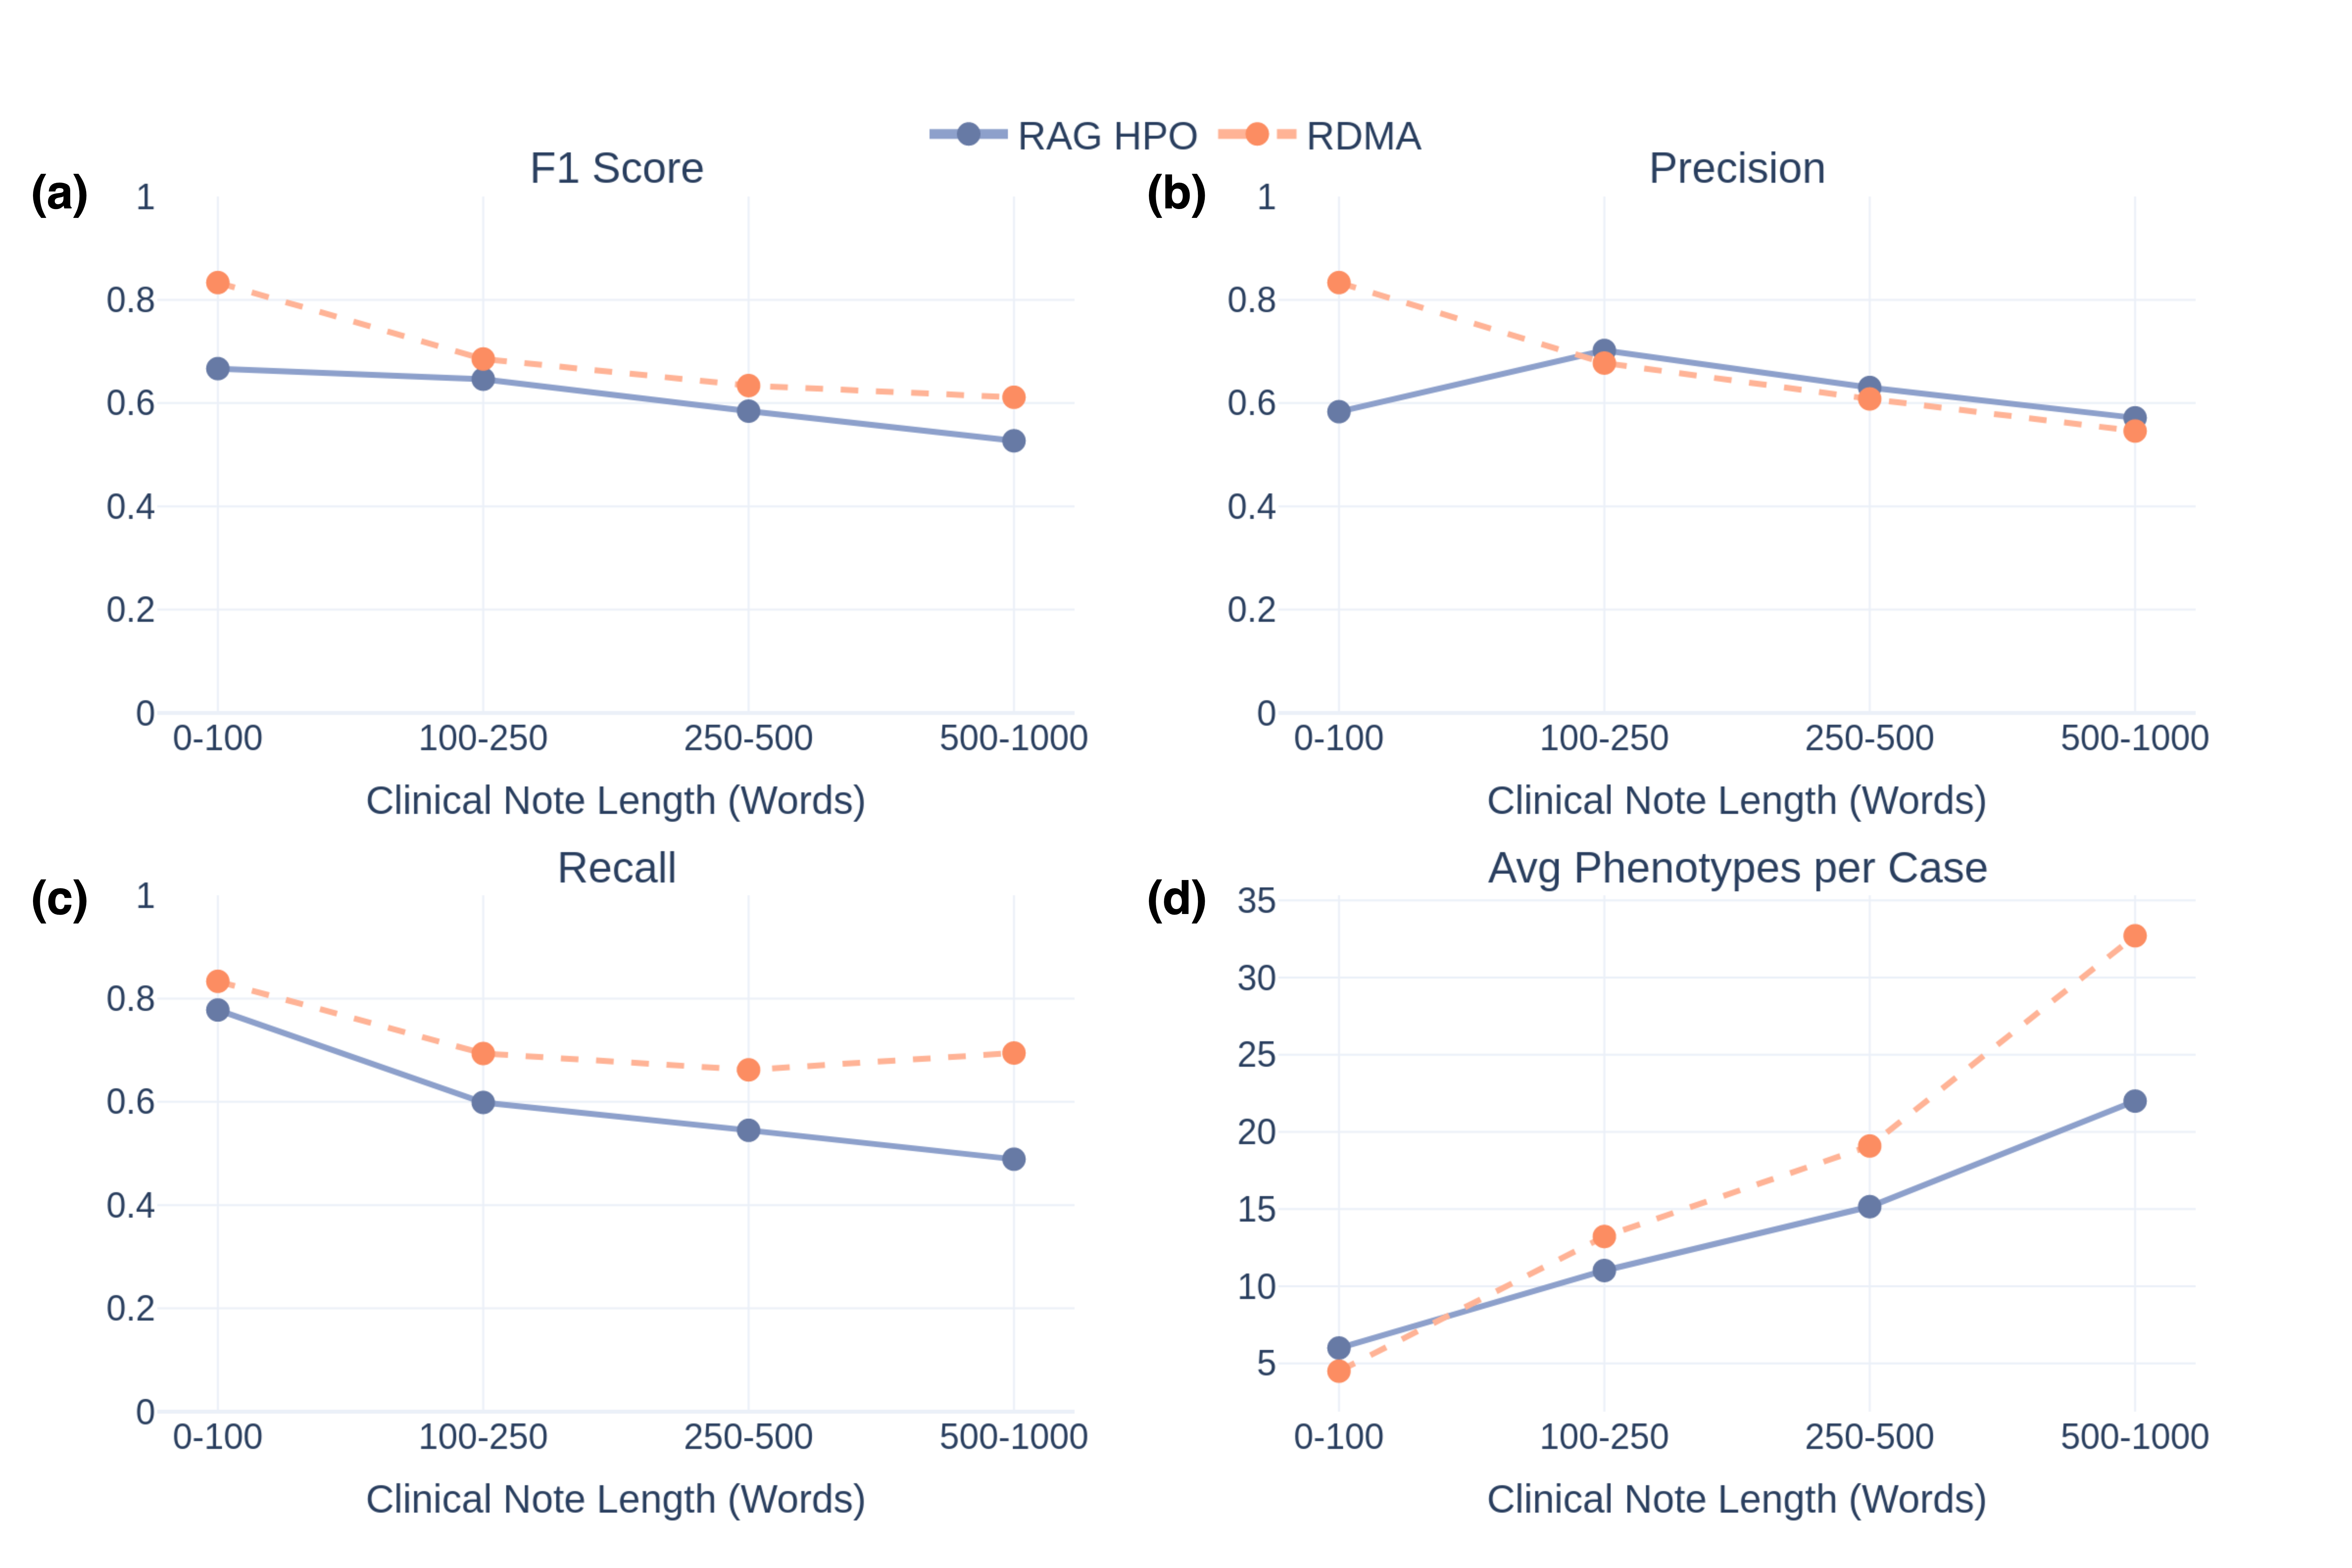
\includegraphics[width=\textwidth]{figs/hpo_metrics_grid_v2.drawio.png}
    \caption{}
    \label{fig:RDMA_Note_Lengths}
\end{figure}

\rev{\textbf{The need for comprehensive rare disease benchmarks.} Current datasets for mining \cite{lobo2017identifying_human_phenotype_terms,garcia2024_HPORAG,martínezdemiguel2021rarediscorpuscorpusannotated} and differential diagnosis (DDx) \cite{chen2024rarebenchllmsserverare,chen2025rareagentsadvancingraredisease, germain2025applyingAI_RD} face significant limitations. Sentence snippets and scientific passages may not reflect the lengthy, noisy nature of EHRs. Furthermore, many DDx benchmarks use ICD codes as ground-truth proxies, which are flawed because they do not capture rare diseases precisely enough and are often missing from the text \cite{mazzucato2023orphacodes_better, cheng-etal-2023-mdace}. Expecting LLMs to perform accurate DDx without the ability to extract all phenotypes reliably is premature. RDMA provides a framework to generate more accurate ORPHA and HPO-based profiles, but the field requires larger, expert-verified datasets that encompass the full diversity of the Orphanet ontology \cite{weinreich2008orphanet} and HPO \cite{gargano2024mode_hpo}. For future work, extending our mining approach with human verification on the entire MIMIC-III \cite{johnson2016mimic3} and MIMIC-IV \cite{johnson2023mimic4} corpus would be ideal. Gold-standard rare disease and phenotype annotations do not currently exist for MIMIC-IV at scale, however, making this a critical next step. }